%
% Honours Report Template
% updated May 2013
%
\documentclass[a4paper,12pt]{article}
\makeatletter
%\renewcommand\paragraph{\@startsection{paragraph}{4}{\z@}%
%{-2.5ex\@plus -1ex \@minus -.25ex}%
%{1.25ex \@plus .25ex}%
%{\normalfont\normalsize\bfseries}}
%\makeatother
%\setcounter{secnumdepth}{4} % how many sectioning levels to assign numbers to
%\setcounter{tocdepth}{4}    % how many sectioning levels to show in ToC
%
\usepackage{url}
\usepackage{epsfig}
\usepackage{latexsym}
\usepackage{graphicx}
\usepackage[square,sort&compress,numbers]{natbib}
% It also sets the bibliographystyle to plainnat; for more information on
% natbib citation styles, see the natbib documentation, a copy of which
% is archived at http://www.jmlr.org/format/natbib.pdf
\usepackage{setspace}
\usepackage{amsmath}
\usepackage{amssymb}
\usepackage{amsfonts}
\usepackage{color}
\usepackage{etaremune}
%stop splitting words at the end of a line
%\usepackage[none]{hyphenat}

%\graphicspath{{./figures/}
%Formatting-------------------------------------------------------------------
%\renewcommand{\refname}{\textbf{Literature}}
%
\renewcommand{\contentsname}{\small\textbf{{\center Table of Contents}}}
%
\setlength{\textheight}{8.8in}
%
\setlength{\topmargin}{-1.5cm}
%
\doublespacing
%\setlength{\textwidth}{17cm}
%
%\setlength{\oddsidemargin}{-0.1714in}
%
% Boxit -----------------------------------------------------------
\setlength{\fboxrule}{0.2mm} \setlength{\fboxsep}{4mm}
%
\newsavebox{\savepar}
\newenvironment{boxit}{\begin{lrbox}{\savepar}
        \begin{minipage}[b]{4.6in}}
        {\end{minipage}\end{lrbox}\fbox{\usebox{\savepar}}}
        
        
        
        
 \hyphenation{op-tical net-works Mathe-ma-tical street-scape street-scapes aes-the-tics aes-the-tic com-pu-ting geo-metric Geo-me-tric geo-metry boun-da-ries de-ve-lop-ment know-ledge mani-fold mani-folds high-di-men-sio-nal}
%
%
%
% Document-----------------------------------------------------------------------
%
\begin{document}
%
\title{\bf SENG4150 - DISTRIBUTED OPERATING SYSTEMS FINAL EXAMINATION}
%
\author{Ross Bille - 3127333\\
School of Electrical Engineering \& Computer Science\\
The University of Newcastle\\ Callaghan NSW 2308, Australia\\
Email: \texttt{c3127333@uon.edu.au} } 

\maketitle
\newpage
\section*{Question 1}

A system of this description would contain a page table size of $2^{55}$~bytes out of the possible $2^{64}$~bytes.
Being multi level means to locate a page we would need to follow a chain of page tables through each layer of the tree that represents the virtual memory (VM).
As each page is 4KB (4096 bytes) and each entry in a page table is 8 bytes, this means that each page can reference 4096/8 pages leaving us with each node of our VM tree having 512 possible leaf nodes.
With this all in mind, if we divide the total size ($2^{64}$ bytes) by the size of a page (4096 bytes) then we can see that we have $2^{52}$ leaf nodes in the tree.
Since $log_2(512) = 9$ we can determine how many parent nodes at each level until we get to the root node whic is fixed in RAM:
\begin{etaremune}
    \item{$2^52$}
    \item{$2^43$}
    \item{$2^32$}
    \item{$2^21$}
    \item{$2^12$}
    \item{$2^3$}
\end{etaremune}
This means that to get to the data that is requested the system has to search 6 tables (Figure~\ref{img:tableGraph}). 
This means there are 6 page table look ups and the possibility of 6 page faults (1 per table that is not the root and 1 to get the data) making less desirable data access times than a system that divides up its memory.

\begin{figure}[ht!]
    \centering
    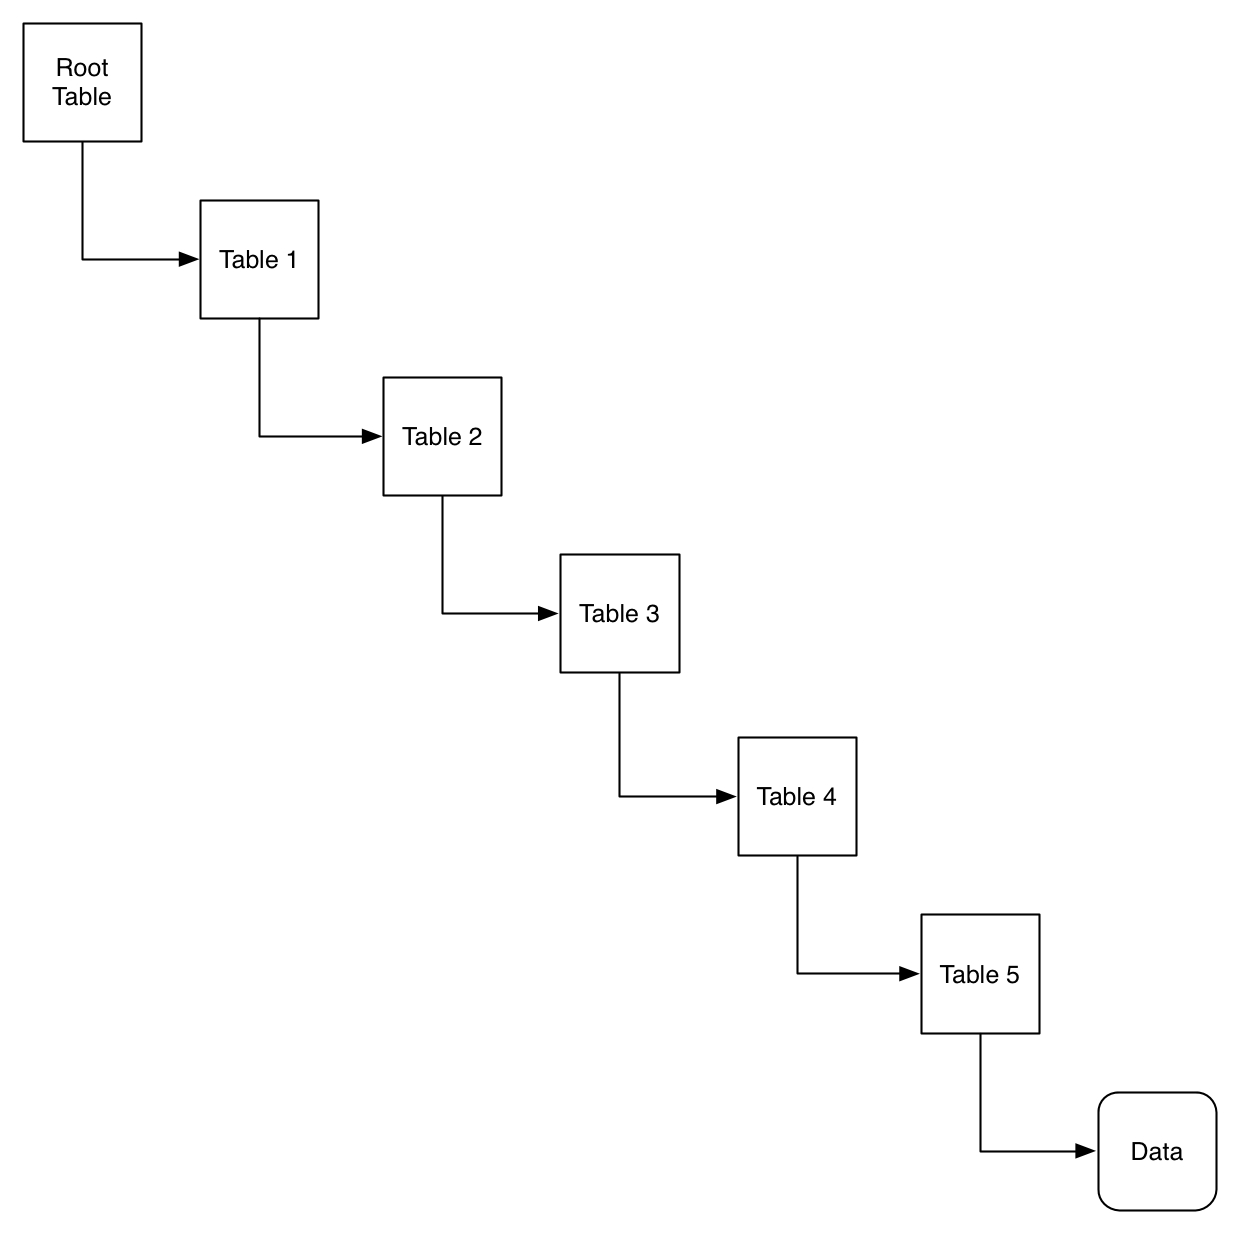
\includegraphics[width=125mm]{./images/PageTables}
    \caption{Tree graph representation}
    \label{img:tableGraph}
\end{figure}
%explain what a multi-level page table is

%

\section*{Question 2}
\subsection*{Identity Incorporating Address}
In this approach (referred to as the IIA approach for the remainder of this exam) the name of each object in the system incorporates its address, such as back in biblical times when people had names like ``Jesus of Nazareth''. 
This system makes it simple to find objects, however this will cause problems when objects are moved.
To follow on from the biblical example above, visiting ``Nazareth'' did always lead finding ``Jesus''.
Just like it is unreasonable to expect a person to stay in the one place, it is unreasonable to expect objects to stay in the one place, objects can be moved for many reasons, such as:
\begin{itemize}
    \item{Move from failing/failed node}
    \item{Physical disk movement}
    \item{}
\end{itemize}

Therefor when implementing this system we need to enforce extra measures, one such measure is chaining. 
When an object is moved from a source to a destination in chaining a forwarding address is left at the source, this allows for future lookups of that object to follow the chain of forwarding addresses until it finds the object it was looking for.

Chaining is still not perfect, if one of the nodes in the chain goes offline then the object can not be accessed even if the node containing the object is online.
It also introduces overhead for objects that have been moved around a lot.

A system that implements the IIA approach is the MONADS system
%What is it
%how it works
\subsection*{OID}
Having a database of objects 
%What is it
%how it works
\subsubsection*{Issues}
\textbf{\indent~Addressing}\\
%size
Generally OIDs are assigned in a hierarchical manner to create a structure logical structure which speeds up access times, one such example of this would be the use of a binary tree.
If this is the approach taken to assign OID's then the act of moving objects becomes a larger issue in this OID approach when compared to the IIA approach.
This is apparent because moving an object would mean having to change its OID, which would mean having to update all the other objects that have a reference to it (which is non-trivial). 

%loosely couple - Well if you move an object in the alternative approach, you only have to change the value of the key. Rather than go through MONADS approach to moving modules
    %MONADS tightly coupoles the VMA to the location, meaning any change in the location, requires all nodes to update in some way
\textbf{\indent~Protection}\\
With a conventional database, permissions may be set at the database level, read and writes are either granted or denied, these permissions are no allocated to anything smaller than a database (rows and columns).
When viewing this implementation of stable store it becomes apparent that security and access control becomes a problem, this is because we cannot simply set a database permission (this would not be sufficient), we would need to set individual object permissions.
This is inefficient and difficult to maintain, with the possibility of $n*(n-1)$ permissions throughout the database.
%security
%Access permissions/control



\section*{Question 3}

\subsection*{Concurrent Access}
%Define Concurrent access
Concurrent access refers to the ability of multiple processes to access systems resources or components simultaneously. 
For instance multiple processes accessing the same message queue at the same time~\citep{managing-concurrent-access}, or multiple processes accessing the same data at the same time.
\subsubsection*{Issues}
%Define the issues that arise due to concurrent access]
Issues can arise in concurrently accessible system because there can exist sets of actions that need to be executed in a specific order to ensure data integrity.
For example purposes I will use the following example of a bank transfer as a set of related actions that need to be executed in the following order:

\begin{center}
    \begin{boxit}
        \begin{center}
               \begin{enumerate}
                    \item{Start}
                    \item{Check bank account A has more than \$500 to deduct}
                    \item{Deduct \$500 from account A}
                    \item{Increase bank account B by \$500}
                    \item{End}
                \end{enumerate}
        \end{center}
    \end{boxit}
\end{center}
\begin{center}
    Example 1 - Actions in a simple bank funds transfer.
\end{center}
None of these actions should be executed if the previous fails and care needs to be taken if other processes need to manipulate the data that these actions are manipulating (i.e. the funds in account A).

\par\textbf{\indent Lost Update}\\
The lost update problem occurs when an update of data is completed by a user but is overridden by another user.
\citep{database-systems}.

\par\textbf{\indent Uncommitted Dependency (dirty read)}\\
The uncommitted dependency problem occurs when a process~(processA) is able to view the results of a separate process~(processB) before the results~(of processB) have been committed~\citep{database-systems}.

\par\textbf{\indent Inconsistent Analysis Problem}\\
The inconsistent analysis problem occurs when a process~(processA) reads several values but a second process~(processB) updates some of those values during (processA's) execution.
In example 1, if bank account A contains \$500 and two sets of these actions are executed at the same time, then step 2 will evaluate true for both executions and account a will have -\$500.

\par\textbf{\indent System Failure}\\
If a system has a failure, such as a power outage, while executing a related set of actions then the system can be put into an invalid state. 
In example 1, if a process runs the execution and the system fails after step 3 then the state will be invalid because \$500 was deducted from account A but account B is never credited.


\subsection*{Transactions}
%define transactions
Transactions were designed to overcome the issues presented above.
A transaction represents a set of related actions that are performed as a unit~\citep{nested-transactions}.
For instance the bank transfer actions listed above represent a single transaction. 

% ACID
For a transaction to be considered effective it must possess the following attributes:
\begin{itemize} 
    \item{Atomicity - All of the actions pass or none do.}
    \item{Consistency - All transactions must leave the data in a correct state.}
    \item{Isolation - Transactions cannot interfere with each other.}
    \item{Durability - Effects of successful transactions must persist even through system failures.}
\end{itemize}
These attributes are known as the ACID properties.

\par\textbf{Transaction Manager}\\
% Transaction Controller
The job of the transaction manager (TM) is to ensure the execution of transaction within the set of resources that is responsible for.
The TM makes sure all transactions adhere to the ACID properties in order to keep the systems is always in a valid state.
Generally to ensure integrity a TM will lock the resource(s) that a transaction is attempting to manipulate until that transaction commits its changes.
There are different rules that a TM will enforce to achieve this locking, two such rules being pessimistic and optimistic, defined below.

\par\textbf{Pessimistic vs. Optimistic Locking}\\
Pessimistic locking assumes the worst~\citep{pessimistic-vs-optimistic}, it assumes that multiple users will want to manipulate the same piece of data at the same time. To avoid conflict, the first time a piece of data is accessed the TM will lock it so no other process can access it.

Optimistic locking assumes that conflicts will be rare and therefor will only perform a lock if it finds evidence that a conflict will occur~\citep{pessimistic-vs-optimistic}.



\subsection*{Effectiveness in Non-Connected  Computers vs. Distributed Operating Systems}
%how they solve above issues
%use of Centralised Transaction controller vs other means of transaction control
In a non-connected computer a single centralised TM is responsible for all transactions in the system. 
This is simple to accomplish because it will have visibility and control over all aspects of the system in which it is contained. 

However when it comes to a distributed operating system a central TM makes little sense. 
In a distributed system there are many owners of many resources that all nodes can have access to.
For a central TM to work all requests of access of these resources must go through this TM before they can be served.
Not only does this create a bottleneck but it also causes a significant single point of failure, this is because the TM would need to live somewhere. 
If we allocate a node for this job and that node goes down then the rest of the system can not function, which is not acceptable in a proper distributed system where the system should still be usable even if a node fails.


An alternative would be to let the owners of each resource act as transaction managers, or by implementing the two phase commit protocol (2PC).
Letting the resource owners act as individual TM's means that if a node goes down the emphasis would be on not being able to access the resources it housed.

\subsubsection*{2PC}
As the name suggests 2PC consists of two phases:
\begin{enumerate}
    \item{Voting phase - All participating processes are told to take steps to prepare for commiting or aborting, each participant must reply with commit or abort (if there has been a problem).}
    \item{Commit phase  The coordinator will instructs all participants to either commit (if all voted commit) or abort and rollback (is any voted abort).}
\end{enumerate}






\vskip 0.2in
\newpage
\bibliographystyle{apalike}
\bibliography{./literature.bib}

\end{document}
